The prototype developed intends to be integrated with a PCB currently being developed by the research group. The PCB consists of five potentiometric channels, allowing for the measurement of potassium ion concentration, and four amperometric channels to allow for glucose and lactate concentration measurements. The potentiometric readings are amplified using an instrumental amplifier, and the amperometric readings are amplified using a transimpedance amplifier, which also converts the current to voltage. An ADS1298, which is a 24-bit resolution analogue-to-digital converter (ADC), receives the input measurements simultaneously and discretises and further amplifies the signals \cite{TexasInstruments2010}. An ATmega328p microcontroller is used and the PCB allows for both SPI (serial peripheral interface) and UART (universal asynchronous receiver-transmitter) data transmission capabilities. The PCB design in summarised in the block diagram in Figure~\ref{fig: PCB block diagram}.

\begin{figure}[H]
\centering
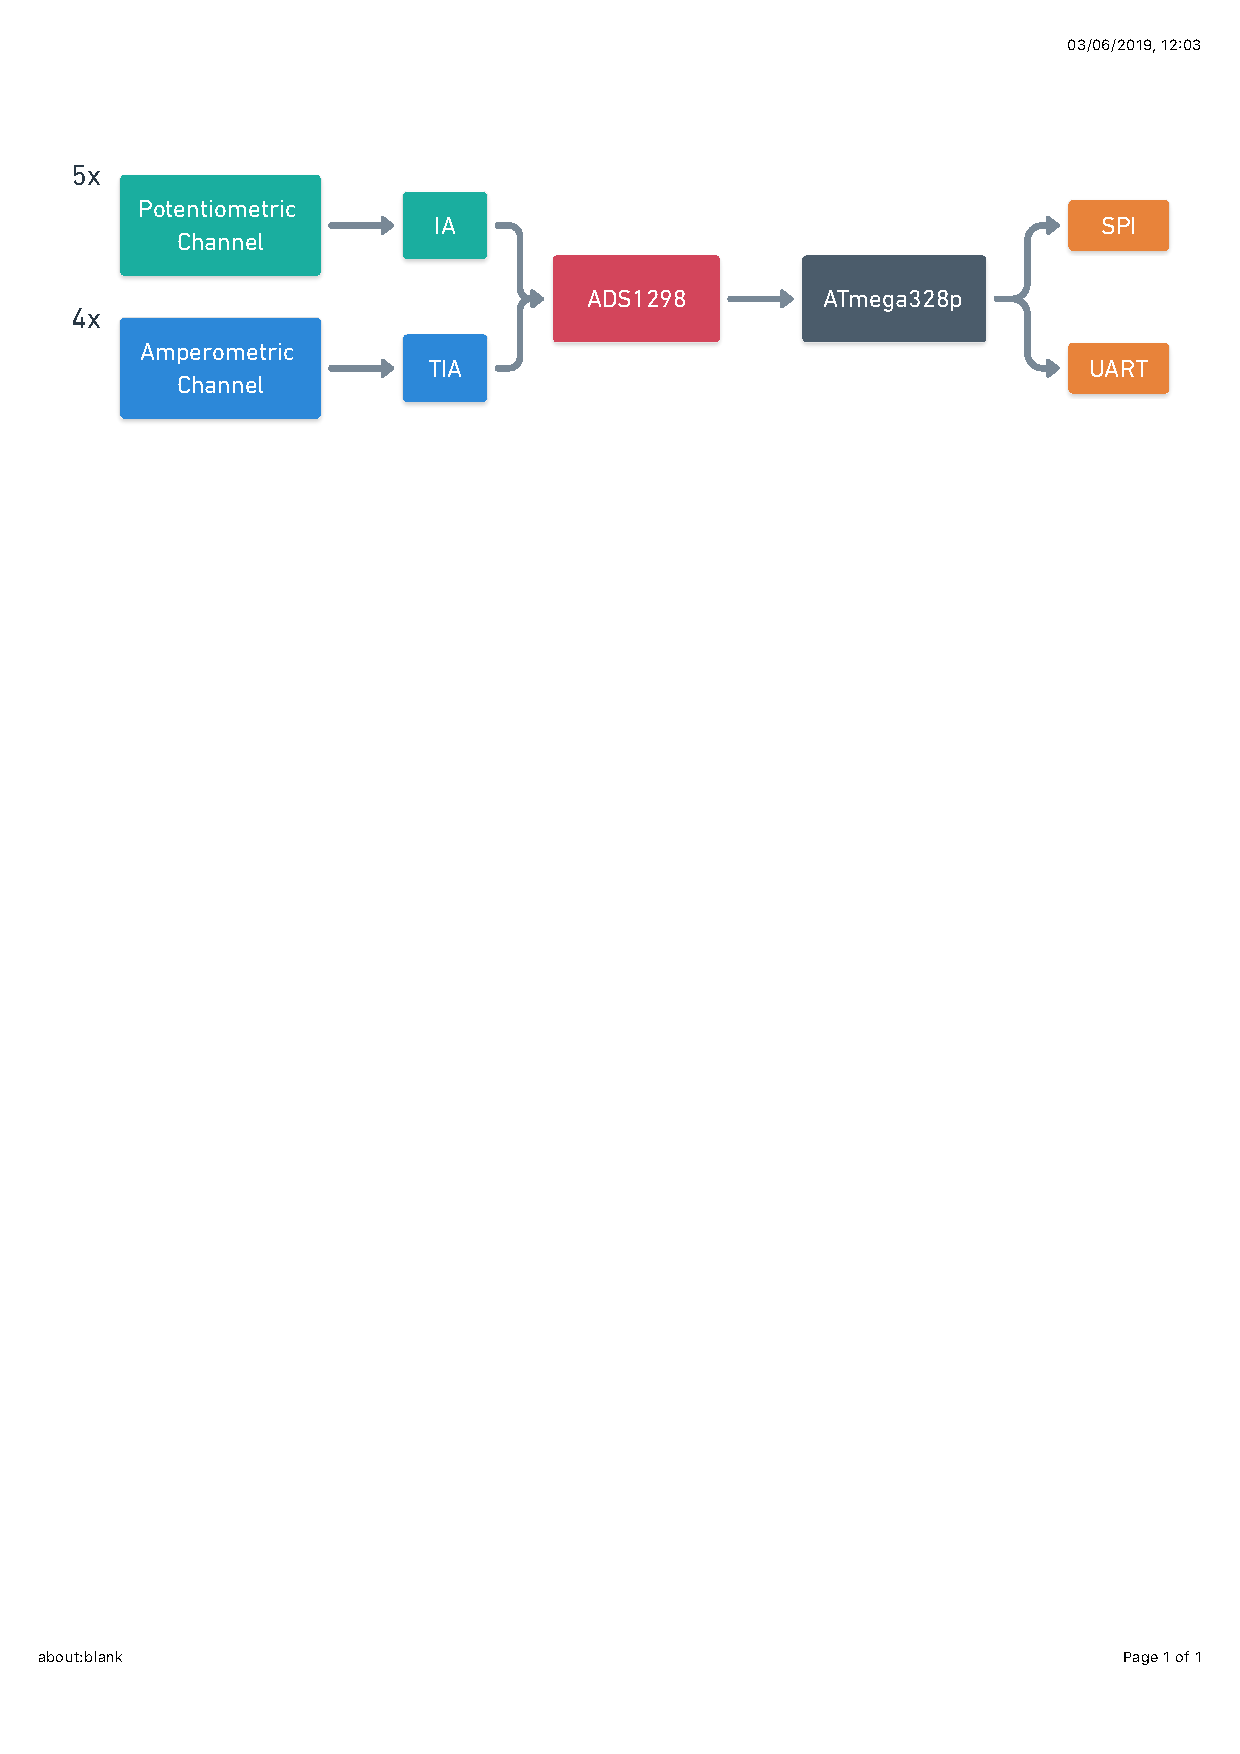
\includegraphics[trim={0cm 22cm 0.5cm  2.5cm}, clip, width=1\textwidth]{./figures/CircuitBlockDiagram.pdf}
\captionsetup{justification=centering}
\caption{Block Diagram of the PCB being developed by the Boutelle Research Group for continuous monitoring of TBI markers}
\label{fig: PCB block diagram}
\end{figure}

The prototype developed is a simplified model of the PCB. The prototype receives three amplified voltage signals, corresponding to glucose, lactate and potassium, so it continues on from the PCB block diagram after the ADS1298. The prototype then extends further from the functionality of the PCB by processing the received signals, developing the wireless transmission of the data and developing an iPad application, as shown in the flowchart in Figure~\ref{fig: flowchart}. The code for this project can be found in Appendix~\ref{appendix: a}.

\begin{figure}[H]
\centering
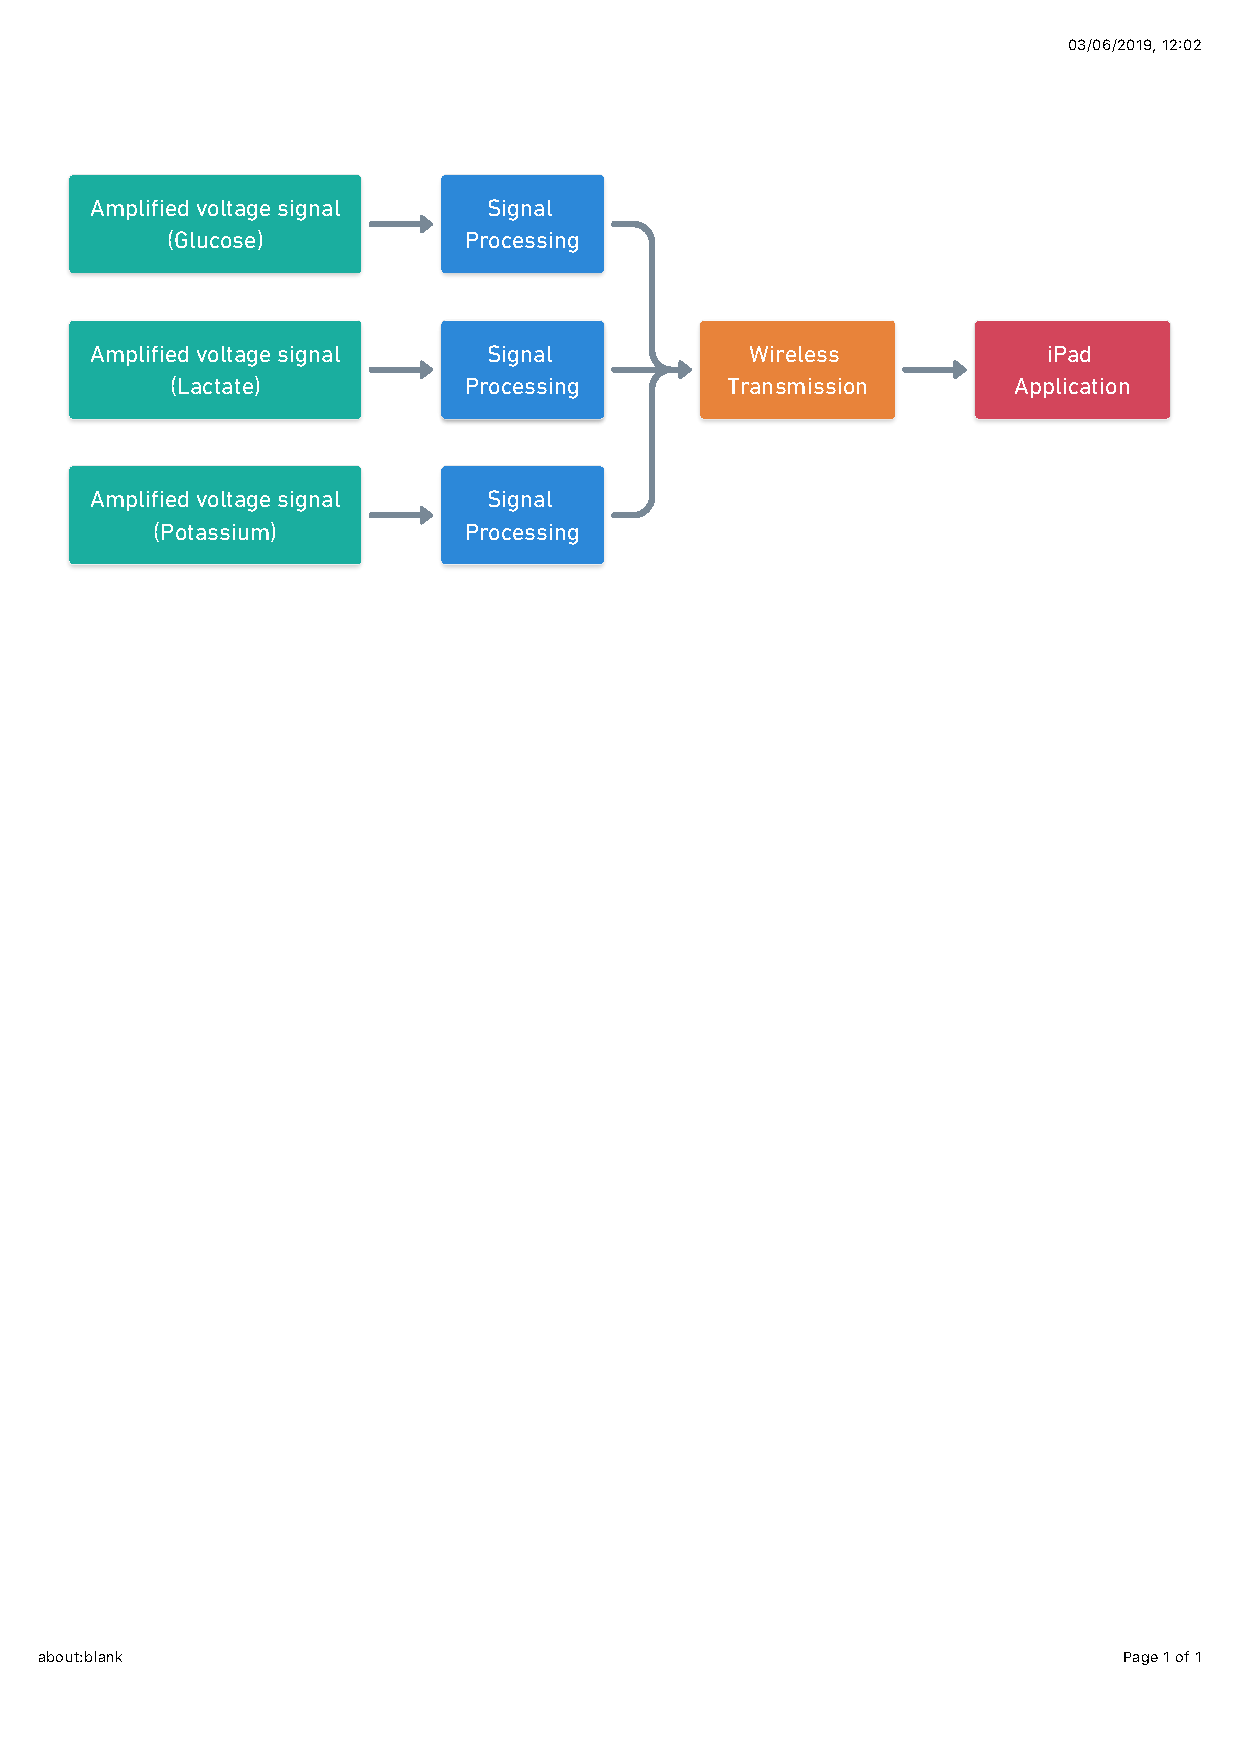
\includegraphics[trim={0cm 19.5cm 0.5cm  2.5cm}, clip, width=1\textwidth]{./figures/Flowchart.pdf}
\captionsetup{justification=centering}
\caption{Flowchart of the key elements in the prototype system}
\label{fig: flowchart}
\end{figure}



\subsection{Hardware}
The hardware of the prototype consists of an Arduino Nano and a Adafruit Bluefruit LE SPI Friend, as shown in Figure~\ref{fig: breadboard}. The Arduino Nano was chosen as a suitable microcontroller for prototyping and mimicking the PCB as it also contains an ATmega328p microcontroller and has an inbuilt ADC. However, the ADC is only 10-bit, so it has poorer precision than the ADS1298. The Arduino is also simple to programme due to the IDE and libraries available, making it suitable for prototyping.

\begin{figure}[H]
\centering
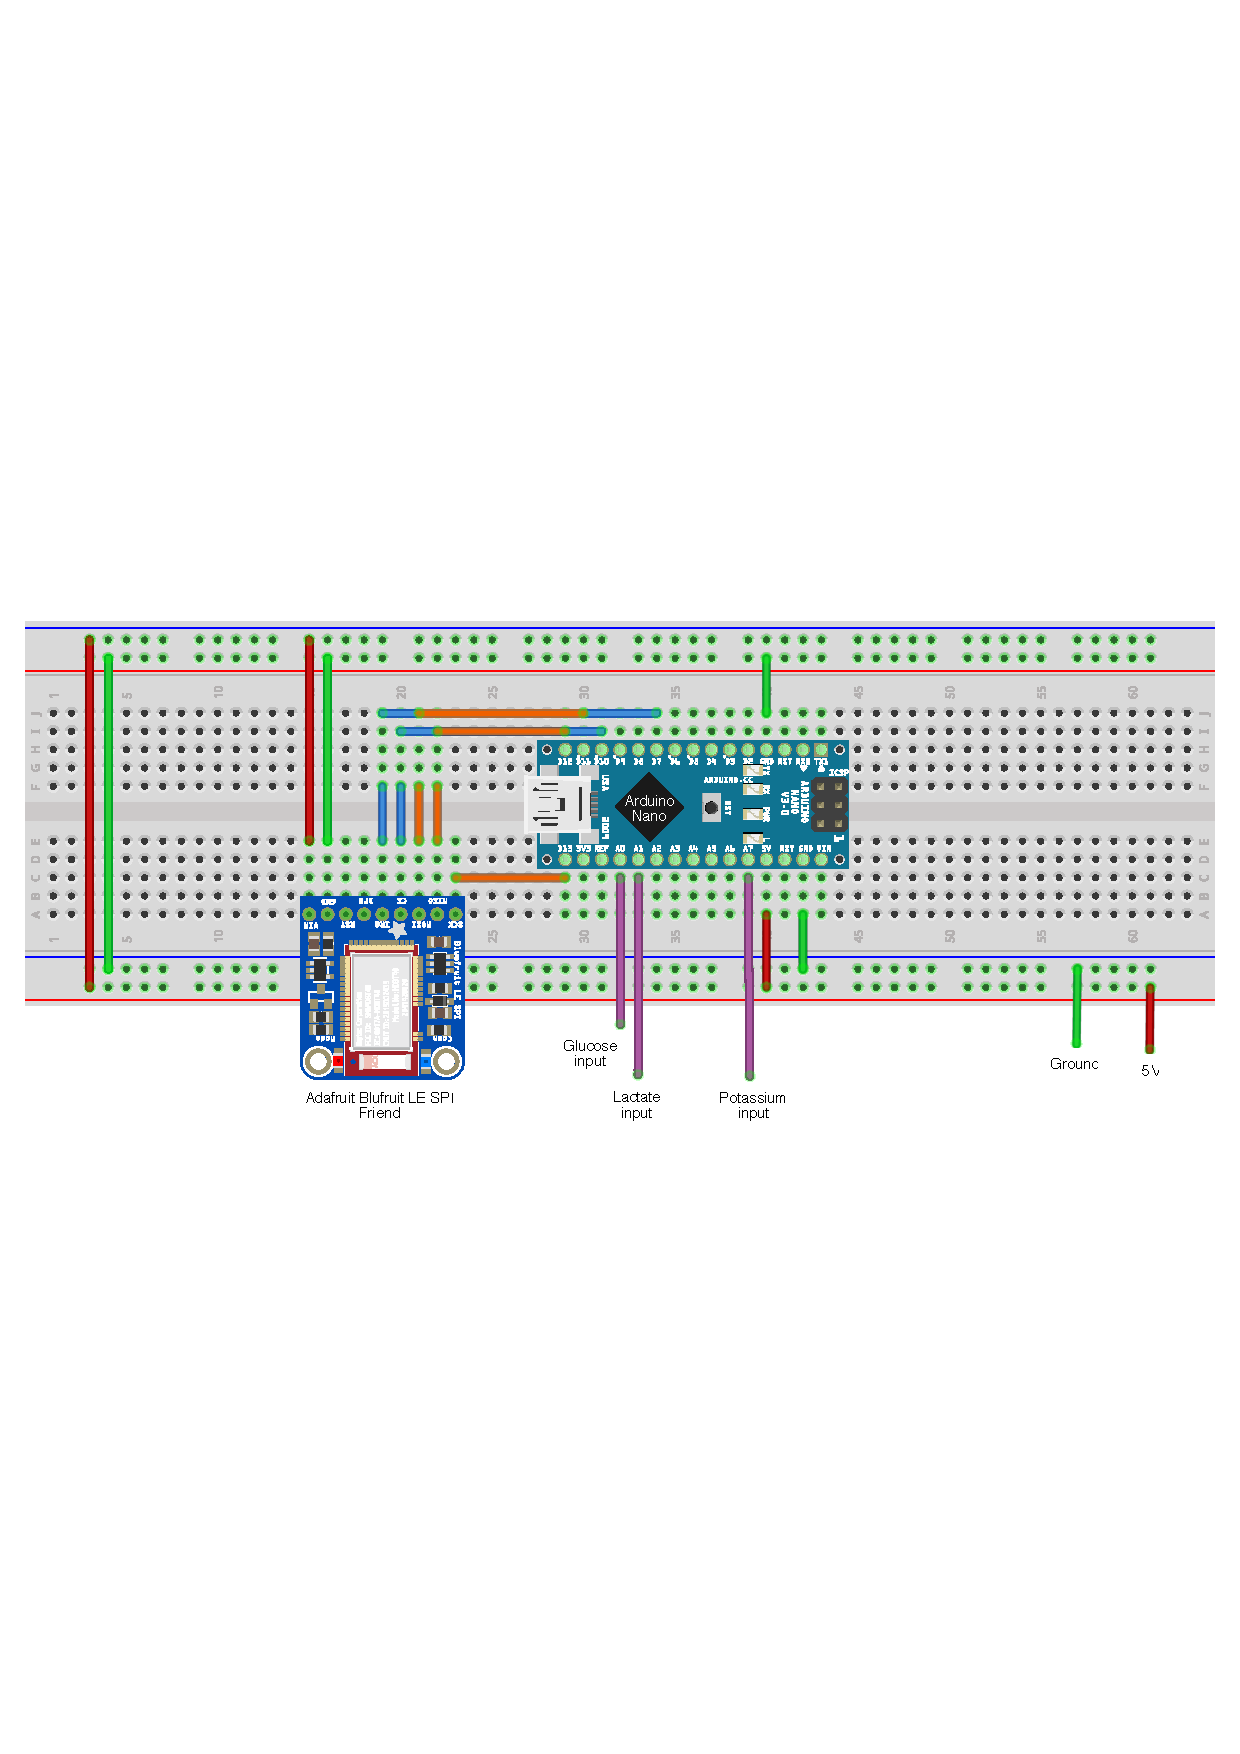
\includegraphics[trim={0cm 10.5cm 0cm  10cm}, clip, width=1\textwidth]{./figures/Breadboard2.pdf}
\captionsetup{justification=centering}
\caption{Prototype assembled on breadboard}
\label{fig: breadboard}
\end{figure}

The Arduino Nano receives three input voltage signals ranging from 0V to 5V at the analogue pins A0, A1, and A7. These input pins correspond to glucose, lactate, and potassium. The signals are discretised by the inbuilt ADC. The Nano records the time at which each signal is read, along with the value of the signal. The signal recordings are processed before being passed to the Bluefruit.



\subsection{Firmware}
The Arduino Nano is encoded to sample and process the three input signals received, then to control the Bluefruit to wirelessly transmit the signals via Bluetooth low energy (BLE). The algorithm encoded in the Arduino is described in Figure~\ref{fig: psuedocode}.


\subsubsection{Signal Processing}
Every 200ms the Arduino reads the input signals at the A0, A1 and A7 pins and records the time at which sampling occurred. The recorded data is mapped to its corresponding voltage value. For every five samples of data recorded, so in a 1s period, the average voltage is calculated for each signal. This averaging methods allows large deviations and spikes to be smoothed, thereby reducing the effect of noise on the outputted data.

Each input signal received by the Arduino is filtered with a low-pass filter with a cut off frequency of 1Hz. This cut off frequency was chosen because the events indicating a SD occur over a long time frame, as shown in Figure~\ref{fig: SD}, hence the changes occur slowly and at low frequency. The low pass filter attenuates high frequency components that may arise from noise or patient movement, allowing for a cleaner signal to be obtained that contains the relevant data.


\subsubsection{Wireless Transmission}

\begin{figure}[t!]
\centering
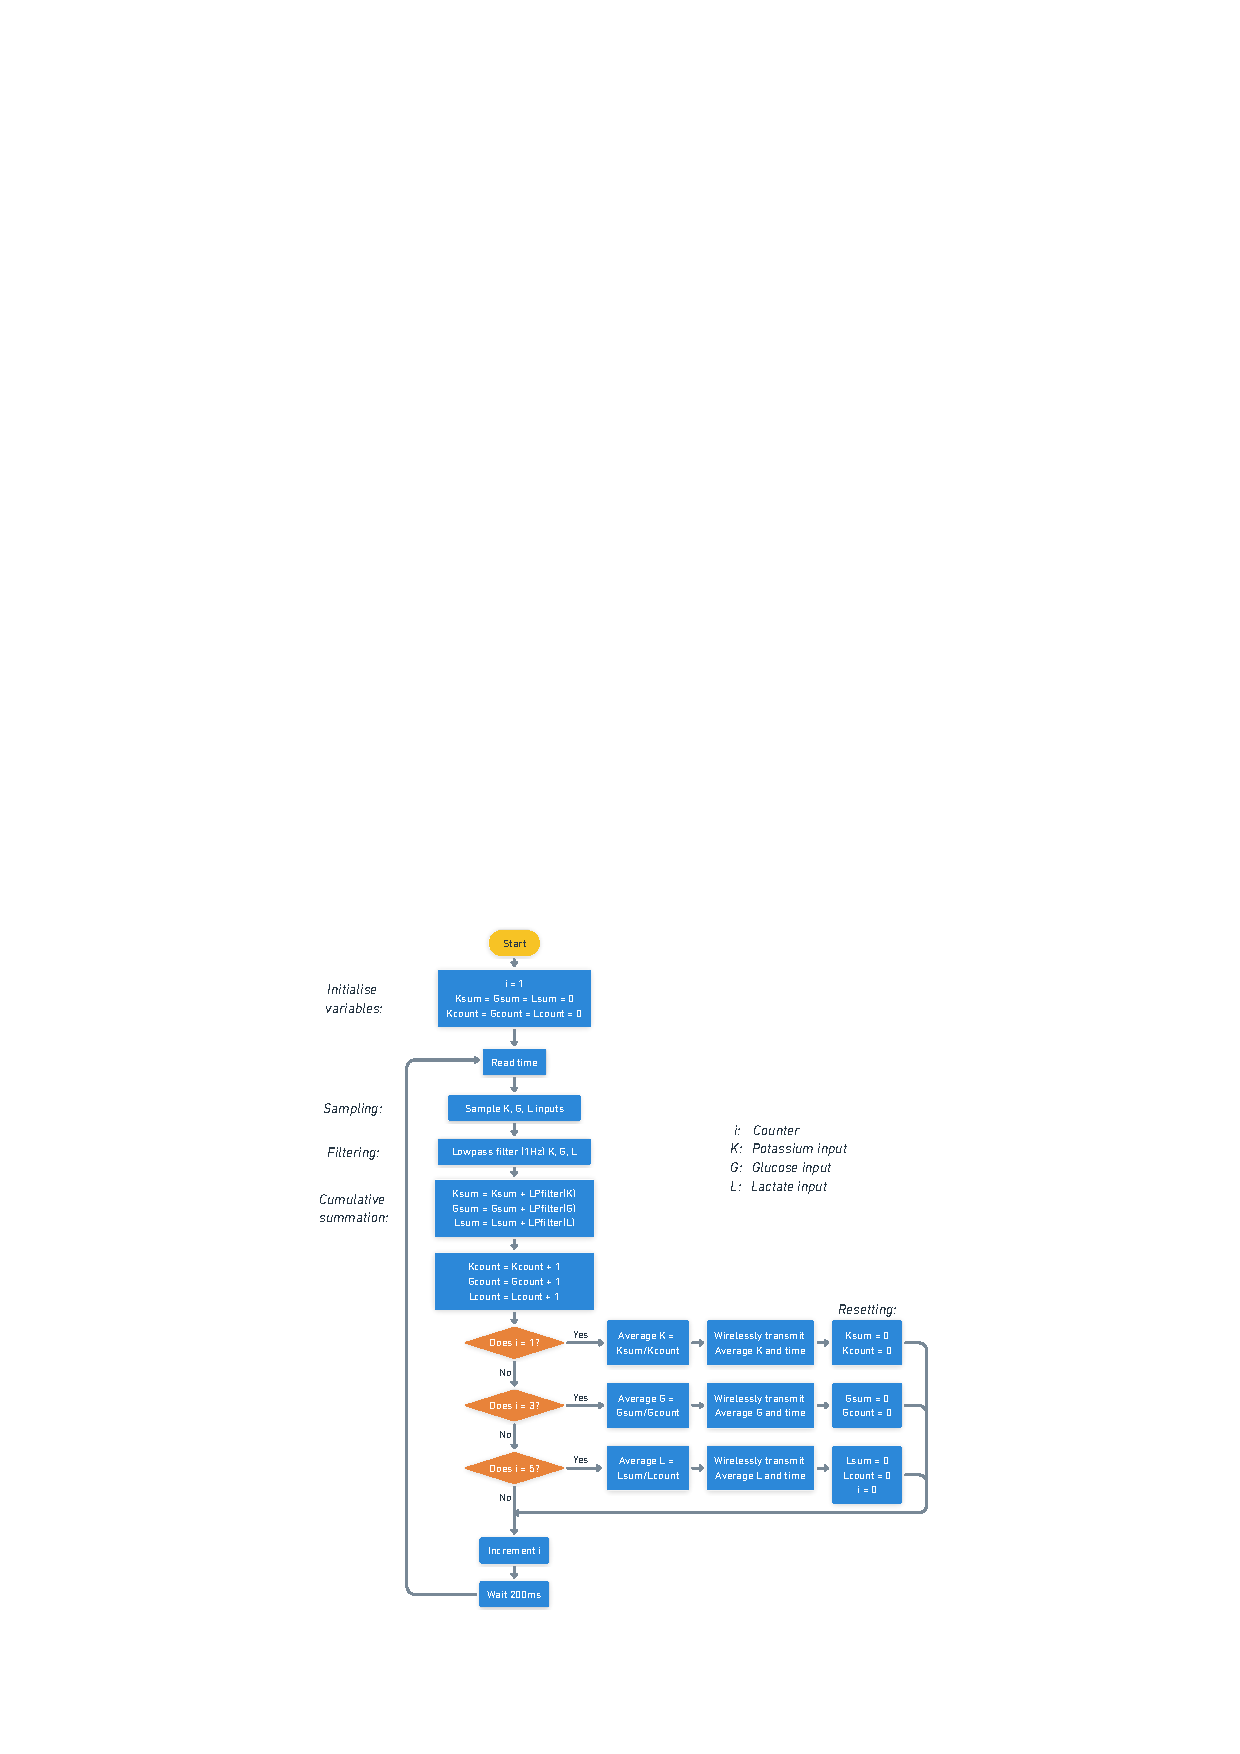
\includegraphics[trim={1cm 5cm 1cm  4cm}, clip, width=1\textwidth]{./figures/psuedocode.pdf}
\captionsetup{justification=centering}
\caption{Flowchart of algorithm encoded in Arduino Nano}
\label{fig: psuedocode}
\end{figure}

Bluetooth Low Energy (BLE) and ZigBee are both popular wireless data transmission options for IoT projects. Table~\ref{table:BLE vs ZigBee} summarises the differences between BLE and ZigBee.

\begin{table}[t!]
\centering
\begin{tabular}{||c c||} 
 \hline
 BLE & ZigBee \\ [0.5ex] 
 \hline\hline
 Short range (77m) & Medium range (291m) \\
 Higher data rate: 1Mbps bursts & Lower data rate: 250kbps \\ 
 PAN (personal area network) & LAN (local area network) \\
 Throughput: 0.27Mbps & Throughput: 0.03Mbps \\
 Latency: 3-6ms & Latency: 15ms \\
 Sleeps between bursts $\rightarrow$ uses less power & No sleep functionality \\
 Supported on most OSs including iOS & Not supported on most OSs \\
 \hline
\end{tabular}
\caption{BLE vs. ZigBee \cite{Ray2015, Christiano}}
\label{table:BLE vs ZigBee}
\end{table}

For this project, BLE is the most suitable option. BLE offers more efficient data transfer and is compatible with iOS. BLE has a shorter range than ZigBee, but this is not of hindrance as the patient will remain close to the iPad that will receive the signals. BLE is commonly used for health and fitness trackers, making it a suitable method of transmission for this project's application.

Adafruit provide a variety of Bluetooth low energy modules that are compatible with Arduino and provide a library that can be used with the Arduino IDE: Adafruit\_BluefruitLE\_nRF51. Adafruit also provide an iOS app to test the bluetooth module and view the received signals. Whilst the PCB currently being developed allows for both SPI and UART data transmission, SPI was the chosen mode for the prototype hence the Bluefruit LE SPI Friend was chosen over the Bluefruit LE UART Friend. Both share similarities and have the same library that is used in the Arduino IDE, however SPI was preferred as it has a clock line where data can be sent along with the clock pulses, so the timing of when data is sent is more reliable. The Arduino Nano has inbuilt SPI pins: D11 is MOSI, D12 is MISO and D13 is SCK. These connect to the corresponding pins on the Bluefruit. D10 on the Arduino is programmed as the CS and D7 is programmed as the IRQ, which are then wired to the corresponding Bluefruit pins. 

The Adafruit\_BluefruitLE\_nRF51 library provides a header file specifically for the Bluefruit LE SPI Friend which provides functions that allow for the transmission of data via BLE to a paired device, such as {\tt{ble.print()}}. The limitation of this function is that a maximum of 20 characters can be sent at a time otherwise the data becomes fragmented. This means that the data from each input pin and the corresponding time of recording has to be wirelessly transmitted one at a time rather than all three simultaneously to prevent the risk of the data fragmenting. The data from each input pin is outputted in characters as:

\begin{align}
    Output = ID + Time + Value + \backslash n.
    \nonumber
\end{align}

The ID at the beginning identifies which signal is being read i.e. G for glucose, and the newline character ($\backslash$n) at the end concludes the data transmission. If both these identifiers are not present at the receiving end, this indicates that the data is fragmented and the receiving app will discard the data. 

Another limitation was observed when all three inputs were periodically sent within a 200ms period. The data would initially be sent correctly but after some time, the data would fragment. The Bluefruit struggled to send data so quickly, which created a backlog of data that was responsible for the fragmentation. Eventually, the Bluetooth module would disconnect from the app. To prevent this, the three signals were periodically sent every 1s, spaced such that potassium was sent at 200ms, glucose at 600ms, and lactate on the 1s. Since the electrochemical changes in the brain occur at slow rates, for example an SD event takes about 10 minutes, a sampling speed of 1s is suitable for this application. 





\subsection{iPad Application}
The iPad app was written in Swift using XCode. The story board is shown in Figure X.
